\subsection{Stability analysis}
\label{subsec:stability_analysis}

As introduced at the beginning this section, a shunting circuit can be either passive or active.
While passive shunts are stable by definition (conservation of energy), active shunts can introduce instabilities in the system.

In particular, considering piezoelectric patches connected to a shunting circuts, two types of instabilities can be introduced:

\begin{itemize}
    \item \textbf{Mechanical instability}: the equivalent stiffness of the piezoelectric patch become negative;
    \item \textbf{Electrical instability}: the equivalent capacitance of the electrical circuit becomes negative.
\end{itemize}

For the sake of simplicity, we consider here only the case of the purely capacitance shunting circuit, with a series connection between the piezoelectric patch and the shunt capacitor (similar to the one shown in Figure \ref{fig:shunt_layouts} (a)).


\subsubsection{$C_N$ shunting circuit}
\label{subsubsec:stability_analysis_negative_capacitance}

As already discussed, the negative capacitance shunting circuit is a particular case of active shunt circuit that can be implemented via OP-AMPs as explained at the beginning of the section.

In this case, considering $Z_{SU} = -\frac{1}{sC_N}$, the mechanical admittance of the piezoelectric patch can be written as:

\begin{equation}
    Y^{SU} = Y_1^D \left( 1 - \frac{k_{31}^2}{1 - C_p^S \frac{1}{C_N}} \right)
\end{equation}

If we consider the ideal case for the shunting circuit, we have already shown in Equation \ref{eq:negative_capacitance_ideal} that the value of $C_N$ doesn't depend on the value of $s = j\omega$.
This means that instability properties (at least in the ideal case) are not frequency-dependent, but rather depends only on the selected value of $C_N$.

In Figure \ref{fig:stability_analysis_negative_capacitance} we show the normalized mechanical admittance of the piezoelectric patch function of the normalized capacitance of the shunting circuit.

\begin{figure}[H]
    \centering
    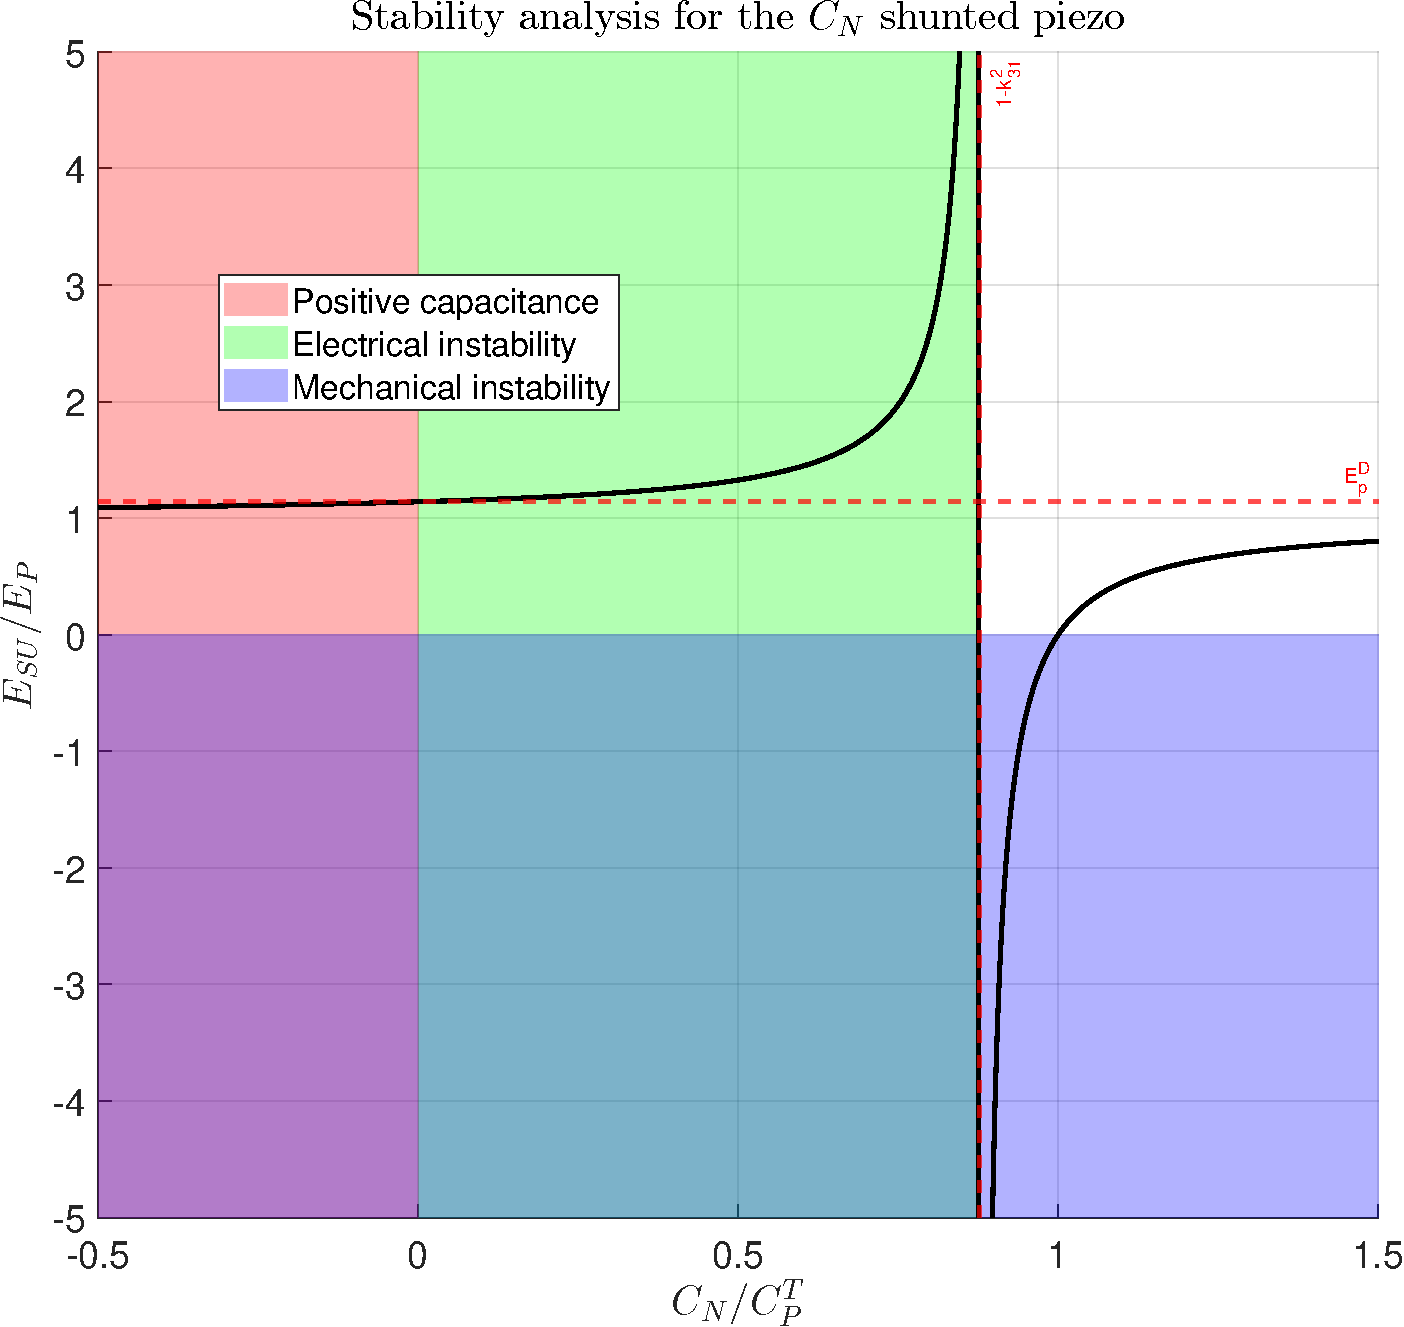
\includegraphics[width=0.5\textwidth]{./img/MATLAB/Stability_analysis_C_N.pdf}
    \caption{Stability analysis of the negative capacitance shunting circuit.}
    \label{fig:stability_analysis_negative_capacitance}
\end{figure}

The colored regions in the plot highlight the regions of mechanical instability (blue) and electrical instability (green).
The red region instead highlights the region where $C_N$ is negative, which means having positive capacitance in the shunting circuit ($C_{eq} = -C_N$).


\paragraph{Mechanical instability}

The mechanical instability region is defined by the condition:

\begin{equation}
    Y^{SU} < 0 \rightarrow 1 - \frac{k_{31}^2}{1 - C_p^S \frac{1}{C_N}} < 0
\end{equation}


\paragraph{Electrical instability}

The electrical instability region is defined by the condition:

\begin{equation}
    C_{tot} = \left( \frac{1}{C_p^T} - \frac{1}{C_N} \right)^{-1} < 0
\end{equation}

Re-arranging the terms, we have:

\begin{equation}
    C_N < C_p^T
\end{equation}


